\documentclass{article}
\usepackage{tenor2015}
\usepackage{times}
\usepackage{ifpdf}
\usepackage[english]{babel}
\usepackage{cite}
\usepackage{microtype}

\usepackage[scaled=0.95]{inconsolata}
\usepackage{verbatim}

\usepackage{listings}
\lstset{language=Python,
showspaces=false,
showtabs=false,
breaklines=false,
showstringspaces=false,
breakatwhitespace=false,
escapeinside={(*@}{@*)},
keywordstyle=\bfseries,
basicstyle=\scriptsize\ttfamily
}

\def\papertitle{The design priorities behind Abjad:
Architecting an open-source software system for Formalized Score Control}
\def\firstauthor{Trevor Ba\v{c}a}
\def\secondauthor{Josiah Wolf Oberholtzer}
\def\thirdauthor{Jeffrey Trevi\~{n}o}
\def\fourthauthor{V\'{i}ctor Ad\'{a}n}

\newif\ifpdf
\ifx\pdfoutput\relax
\else
   \ifcase\pdfoutput
      \pdffalse
   \else
      \pdftrue
\fi

\ifpdf % compiling with pdflatex
  \usepackage[pdftex,
    pdftitle={\papertitle},
    pdfauthor={\firstauthor, \secondauthor, \thirdauthor, \fourthauthor},
    bookmarksnumbered, % use section numbers with bookmarks
    pdfstartview=XYZ % start with zoom=100% instead of full screen;
                     % especially useful if working with a big screen :-)
   ]{hyperref}
  %\pdfcompresslevel=9

  \usepackage[pdftex]{graphicx}
  % declare the path(s) where your graphic files are and their extensions so
  %you won't have to specify these with every instance of \includegraphics
  \graphicspath{{./figures/}}
  \DeclareGraphicsExtensions{.pdf,.jpeg,.png}

  \usepackage[figure,table]{hypcap}

\else % compiling with latex
  \usepackage[dvips,
    bookmarksnumbered, % use section numbers with bookmarks
    pdfstartview=XYZ % start with zoom=100% instead of full screen
  ]{hyperref}  % hyperrefs are active in the pdf file after conversion
  \usepackage[dvips]{epsfig,graphicx}
  \graphicspath{{./figures/}}
  \DeclareGraphicsExtensions{.eps}
  \usepackage[figure,table]{hypcap}
\fi

\hypersetup{
    colorlinks,
    citecolor=black,
    filecolor=black,
    linkcolor=black,
    urlcolor=black
}

%\title{\papertitle}
\title{The design priorities behind Abjad: \\
Architecting an open-source software system \\
for Formalized Score Control}

\fourauthors
  {\firstauthor} {Harvard University \\
    {\tt \href{mailto:trevor.baca@gmail.com}
        {trevor.baca@gmail.com}}}
  {\secondauthor} {Harvard University \\
    {\tt \href{mailto:josiah.oberholtzer@gmail.com}
        {josiah.oberholtzer@gmail.com}}}
  {\thirdauthor} {Carleton College \\
    {\tt \href{mailto:jeffrey.trevino@gmail.com}
        {jeffrey.trevino@gmail.com}}}
  {\fourthauthor} {
    {\tt \href{mailto:vctradn@gmail.com}
        {vctradn@gmail.com}}}

\begin{document}

\capstartfalse
\maketitle
\capstarttrue

\begin{abstract}
abstract goes here and concisely summarizes structure of entire paper
\end{abstract}

\section{Introduction} \label{sec:background}
Abjad\footnote{www.projectabjad.org} is an interactive open-source software
system designed to help composers build up complex pieces of music notation in
an iterative and incremental way.  Abjad is implemented in the
Python\footnote{www.python.org} programming language and architected as an
object-oriented collection of packages, classes and functions. Composers can
visualize their work as publication-quality score at all stages of the
compositional process using Abjad's interface to the
LilyPond\footnote{www.lilypond.org} music notation package. Although the first
versions of Abjad were implemented in 1997 and the project website is now
visited thousands of times each month, we have never documented the design
priorities that have guided us as we have built the system. In this paper we
detail some of the most important principles we have followed in our work
architecting Abjad. The priorities we document here arise in answer to
domain-specific questions of music modeling (what are the fundamental elements
of music notation? which elements of music notation should be modeled
hierarchically? which programming constructs are available to help model the
temporal relationships arising between entities in musical score?) as well as
in consideration of the ways in which best practices taken from software
engineering can apply to the development of a music software system like ours
(which programming concepts concerning things like iteration, aggregation and
encapsulation make sense to make available to composers? which existing tools
to test, document and deploy other open-source projects are available to help
develop a music software system like Abjad?). In the sections that follow we
discuss the background and motivations that lead us to ask questions like these
and then elaborate the design priorities we have arrived at in our ongoing work
architecting Abjad.
\section{Background} \label{sec:background}

While many environments for both notation and sound production been been
created within the last twenty years, the following discussion focuses solely
on the production of notation: Abjad enables composers to express both low- and
high-level compositional ideas by extending a widely used programming language
with a detailed object model of common practice musical notation. To minimize
the restriction of artistic thought's infinite possibility while maximizing the
ability to specify elegantly any arbitrary symbolic relationship, Abjad does
this without prescribing explicit or implicit models of music or composition:
Abjad defines composition narrowly as the act of creating a document via the
encoded aggregation of notational symbols.

\subsection{Generative Task as an Analytic Framework}

Software production exists as an organizationally designed feedback loop
between production values and implementation \cite{Derniame:1999fk}, and it is
possible to understand a system by understanding the purpose for which it was
initially designed, the system's \emph{generative task(s)}. In the analysis of
systems created for use by artists, this priority yields a dilemma instantly,
as analyses that explain a system's affordances with reference to intended
purpose must contend with the creative use of technology by artists: a system's
intended uses might have little or nothing in common with the way in which the
artist finally uses the technology. For this reason, the notion of generative
task is best understood as an explanation for a system's affordances, with the
caveat that a user can nonetheless work against those affordances to use the
system in novel ways. Generative tasks --- informed by the cultural milieu of
software development, economic constraints of software production, and the
aesthetic proclivities of artists participating in development processes ---
constrain software features to enable a limited subset of possible
representations and user interactions.

While composers working traditionally may allow intuition to substitute for
formally defined principles, a computer demands the composer to think formally
about music \cite{Xenakis:1992rq}. Keeping in mind generative task as an
analytical framework, it is broadly useful to bifurcate a  notation
system's development into the modeling of composition, on the one
hand, and the modeling of musical notation, on the other. All systems model
both, to greater or lesser degrees, often engaging in the ambiguous or implicit
modeling of composition while focusing more ostensibly on a model of
notation, or focusing on the abstract modeling of music without a considered
link to a model of notation. Due to the intimate link between notation and
musical ideas, it is impossible for a system that models notation to avoid at
least implicitly modeling musical and compositional ideas, and a computational
model of music and composition is an inevitable component of every
notation system, even when it exists as an unspoken set of technological
constraints. Generative task explains a given system's balance between
computational models of music/composition and notation by assuming a link
between intended use and system development.

\subsection{Computational Models of Notation}

Many systems implement detailed models of composition explicitly or implicitly,
but few of these implement detailed models of notation.\footnote{Computational
models of music might entail the representation of higher-level musical
entities apparent in the acts of listening and analysis but absent in the
symbols of notation themselves, as determined to be creatively exigent.
Programming researchers and musical artists have modeled many such
extrasymbolic musical entities, such as large-scale form and transition
\cite{polansky1991morphological}, \cite{uno1994temporal},
\cite{dobrian1995algorithmic}, \cite{abrams1999higher}, \cite{Yoo1983}, texture
\cite{Horenstein:2004kx}, contrapuntal relationships \cite{Boenn:2009oq},
\cite{Acevedo2005}, \cite{Anders:2011kl}, \cite{Balser:1990tg},
\cite{Jones:2000hc}, \cite{uno1994temporal}, \cite{Bell:1995ij},
\cite{farbood2001analysis}, \cite{Cope:2002fv}, \cite{Laurson:2005dz},
\cite{Polansky:2011fu}, \cite{Ebcioglu:1980kl}, harmonic tension and resolution
\cite{Melo2003}, \cite{Wiggins1999}, \cite{Foster:1995qa}, melody
\cite{Hornel:1993mi}, \cite{Smith:1992pi}, meter \cite{Hamanaka:2005ff}, rhythm
\cite{Nauert2007}, \cite{Degazio:1996lh}, \cite{Collins:2003bs}, timbre
\cite{Xenakis:1991fu}, \cite{Creasey:1996ye}, \cite{Osaka2004}, temperament
\cite{Seymour:2007qo}, \cite{Graf:2006il}, and ornamentation
\cite{Ariza:2003zt}, \cite{Chico-Topfer:1998jl}. This work overlaps fruitfully
with analysis tasks, and models of listening and cognition can enable novel
methods of high-level musical structures and transformations, like dramatic
direction, tension, and transition between sections \cite[108]{Collins2009}.}
Many notation systems --- such as Finale, Sibelius, SCORE \cite{Smith:1972mw},
Igor, Berlioz, Lilypond \cite{Nienhuys:2003ve}, GUIDO \cite{Hoos:1998bd}
NoteAbility \cite{hamel1noteability}, and Nightingale --- exist to help people
engrave music; because these systems provide functions that operate on
notational elements, hidden models of musical notation must underly all of
these systems. Each system's interface constrains and directs the ways in which
users interact with the system's underlying model of notation. These systems
enable users to engrave and format music without explicitly affording the
computational modeling of composition. These tools provide interfaces to
detailed models of notation without allowing equivalently detailed models of
composition, although such systems might go so far as to enable scripting, as
in the case of Sibelius's ManuScript \cite{Technology:qc} scripting language or
Lilypond's embedded Scheme code.\footnote{An attempt to more comprehensively
survey the history of object-oriented notation systems for composition, in the
context of the broader history of object-oriented programming, lies beyond the
scope of this paper but has recently been undertaken elsewhere
\cite{trevino2013compositional}.}

Other systems strike different balances between notation and composition
modeling. OpenMusic \cite{Assayag:1999sw}, PWGL \cite{Laurson:2009qf}, and BACH
\cite{agostini2013real} invite the user to create detailed models of
composition and notation, often with the aid of the above notation editors for
final engraving and layout via intermediate file formats. Some composers use
drawing software like AutoCAD and Adobe Illustrator to create notations; these
provide neither a model of notation nor a model of composition to the user.
Many audio-focused environments afford models of composition without inviting
or providing models of notation \cite{Ariza2005b}. Many systems depend on the
MIDI protocol for output or interchange and cannot provide a hierarchical,
detailed model of notation: for example, if a composer requires a notation
system to render complex rhythmic ideas that depend typographically on nested
tuplets, a system that produces a notation only via a combination of MIDI and
quantization must reduce rhythms to a non-hierarchical stream of event times,
eliminating the temporally divisive approach of tuplet notation previously
modeled.

Many models of musical notation have been designed for purposes of
corpus-based computational musicology. Formats such as DARM, SMDL,
HumDrum, and MuseData model notation with the generative task of searching
through a large amount of data \cite{Selfridge-Field:1997ud}. Commercial
notation software developers attempted to establish a data interchange standard
for optical score recognition (NIFF) \cite{niff1995niff}. Since its release in
2004, MusicXML has become a valid interchange format for over 160 applications
and maintains a relatively application-agnostic status, as it was designed with
the generative task of acting as an interchange format between variously tasked
systems \cite{Good:2001if}.

\section{Extension, not reinvention} \label{sec:extension}

Abjad is not a stand-alone application. Nor is Abjad a programming language.
Abjad is instead an extension to the Python programming language. Our
insistence on this principle of extension --- of adding functionality to an
existing programming language rather than inventing yet another domain-specific
language --- originates in the belief that there is no benefit to be had in
reestablishing the ways variables are created, references are handled, loops
are structured or any of the other fundamentals of programming. We have instead
architected Abjad in the form of a Python package designed to be used the same
way as the thousands of other packages that already exist.\footnote{See the
Python Package Index for functionality to extend the language for purposes as
diverse as creative writing and aeronautical engineering. The Python Package
Index contains 54,306 packages at the time or writing and is available at
\textit{pypi.python.org}.} Even though we find Python an excellent programming
language for architecting a music software system like Abjad,\footnote{Aspects
of Python we find particularly helpful include the availability of lists,
dictionaries and sets as built-in types; the interface provided for string and
Unicode objects; the unified approach to encapsulation provided by Python's
understanding of namespaces; and the extensive functionality provided in the
standard library.} our decision to implement Abjad in Python does not arise
from the specifics of the language but from the fact that the language is part
of a global programming mainstream with tools and best practices that can be
borrowed directly into music composition. In designing Abjad as an extension to
Python, we hope to make relevant the hundreds of print and Web resources that
detail the language and its features. We also hope to make the global community
of developers working in Python available to composers.

\begin{comment}
We hope both benefits will ease composers' transition to
programming and make working with Abjad a familiar task that conforms to widely
understood programming best practices: there will probably by necessity always
be more programmers than composers in the world and it makes sense for our work
as composers to benefit from the patterns already understood elsewhere in the
culture.
\end{comment}

\begin{comment}
source. The history of music software systems is littered with projects that
fell into disuse. Music software systems except for the large commercial
notation packages will probabaly always be the niche efforts of specialists and
our experience architecting Abjad leads us to think about the future in such a
way that we give ourselves all the advantages of expansiveness that are
possible: picking an existing language that makes learning preliminaries
easier and makes the continued development of the system as open as possible to
as many different collaborators as possible.
\end{comment}

\section{An example use session} \label{sec:illustration}

We believe it is important for composers to be able to illustrate the objects
they work with as they compose. Abjad reflects this priority in its
\emph{illustration protocol}.\footnote{Python describes common informal
interfaces to working with objects as \emph{protocols}. Important protocols
include the \emph{iterator protocol} for iterating over the contents of a
container-like object, the \emph{sequence protocol} for getting items and
length from a container-like object and the \emph{mutable container protocol}
for mutating the contents of a container-like object.} Abjad's illustration
protocol conventionalizes the way developers equip Abjad classes with
illustration output and the way composers access illustration output during
composition. The composer-facing part of the protocol is implemented in Abjad's
top-level \texttt{show()} function, which provides composers a unified way to
illustrate any object in the system. The developer-facing part of Abjad's
illustration protocol is evidenced in the collection of
\texttt{\_\_illustrate\_\_()} methods that define how classes throughout the
system are to illustrate when passed to \texttt{show()}.\footnote{Abjad's
pairing of a single \texttt{show()} function with \texttt{\_\_illustrate\_\_()}
methods defined as needed parallels the way Python's \texttt{len()} function
works with \texttt{\_\_len\_\_()} methods defined on custom classes.} Under the
most common pattern, Abjad transforms an object into LilyPond input code and
then calls LilyPond to render the resultant input as a PDF. In all cases the
composer's interface to the illustration logic implemented on a  class is
provided by \texttt{show()}, as in the examples in this
article.\footnote{Abjad's illustration protocol decouples illustration logic
from the other functions of a class. An important consequence of this is that
developers can illustrate classes with LaTeX or GraphViz or any collection of
applications, whether or not LilyPond is included in the tool chain. We find
LilyPond superior for a formalized score control system like Abjad for many
reasons, ranging from LilyPond's powerful model of rhythmic timekeeping to the
high quality of LilyPond output. But should the need arise to replace LilyPond
with a different typesetting engine, the composer-facing  interface provided by
\texttt{show()} will remain the same. The priority is that composers be able to
illustrate compositional objects. LilyPond simply happens to be the best
resource available to achieve our goals.}

\begin{comment}
<abjad>
from abjad import *
note = Note("c'4")
show(note)
</abjad>
\end{comment}

%%% ABJADBOOK START %%%
\begin{lstlisting}
>>> from abjad import *
>>> note = Note("c'4")
>>> show(note)
\end{lstlisting}
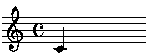
\includegraphics{assets/lilypond-c018a545d264ff34225e9a3a5babb6c1.pdf}
%%% ABJADBOOK END %%%

While most of the examples shown in this paper are demonstrated in Python's
interactive console, Python code --- including Abjad --- is almost always
written as functions and classes in packages and modules to be imported in
other Python code or executed from the commandline.

\begin{comment}
<abjad>[strip_prompt=true]
def make_nested_tuplet(
    tuplet_duration,
    outer_tuplet_proportions,
    inner_tuplet_subdivision_count,
    ):
    outer_tuplet = Tuplet.from_duration_and_ratio(
        tuplet_duration, outer_tuplet_proportions)
    inner_tuplet_proportions = \
        inner_tuplet_subdivision_count * [1]
    last_leaf = outer_tuplet.select_leaves()[-1]
    inspector = inspect_(last_leaf)
    right_logical_tie = inspector.get_logical_tie()
    right_logical_tie.to_tuplet(inner_tuplet_proportions)
    return outer_tuplet
</abjad>
\end{comment}

%%% ABJADBOOK START %%%
\begin{lstlisting}
def make_nested_tuplet(
    tuplet_duration,
    outer_tuplet_proportions,
    inner_tuplet_subdivision_count,
    ):
    outer_tuplet = Tuplet.from_duration_and_ratio(
        tuplet_duration, outer_tuplet_proportions)
    inner_tuplet_proportions = \
        inner_tuplet_subdivision_count * [1]
    last_leaf = outer_tuplet.select_leaves()[-1]
    inspector = inspect_(last_leaf)
    right_logical_tie = inspector.get_logical_tie()
    right_logical_tie.to_tuplet(inner_tuplet_proportions)
    return outer_tuplet
\end{lstlisting}
%%% ABJADBOOK END %%%

\begin{comment}
<abjad>
tuplet = make_nested_tuplet((7, 8), (3, -1, 2), 3)
show(tuplet)
</abjad>
\end{comment}

%%% ABJADBOOK START %%%
\begin{lstlisting}
>>> tuplet = make_nested_tuplet((7, 8), (3, -1, 2), 3)
>>> show(tuplet)
\end{lstlisting}
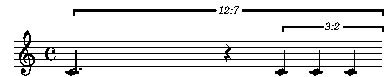
\includegraphics{assets/lilypond-4926e77647583925d3a89653f8577025.pdf}
%%% ABJADBOOK END %%%

\section{The Abjad object model}

Abjad models musical score in terms of \emph{components}, \emph{spanners} and
\emph{indicators}. These families of objects represent all of the notational
primitives in Abjad. Abjad defines components equal to notes, rests and chords
taken together with the container-like elements of music notation, such as
tuplets, measures, voices, staves and complete scores.\footnote{Abjad uses term
`leaf' to generalize notes, rests and chords. The term is borrowed from graph
theory and references the fact that notes, rests and chords can not be made to
contain any other elements of music notation.} Components are arranged
hierarchically into a tree, with containers used to group components
together. Spanners model musical constructs such as beams, slurs
and glissandi which can cross different levels of hierarchy in the score tree.
Indicators model objects attached to a single component. These include
articulations, time signatures, dynamics, and tempo and textual
indications.\footnote{Indicators can have \emph{scope} making them
\emph{effective} for all other components in that scope following the component
to which that indicator is attached until another indicator of the same type
appears. Indicator scoping models how all notes in a voice can be marked as
\emph{forte} until another note is marked as \emph{piano}. We have generalized
the scoping behavior of indicators, allowing composers to annotate score
structures by attaching arbitrary non-notating objects like dictionaries or
custom classes to any component.}

\section{Bottom up construction} \label{sec:bottom-up}

% Abjad never obscures the individual notational elements of the compositional process.

Abjad affords composers the ability to build scores from the bottom up.
Composers work bottom-up when creating individual notes, rests and chords that
are then grouped together into tuplets, measures and voices and nested into the
largest elements of musical structure, like staves and complete scores.

%Composers usually attach spanners and indicators to 
%Any score modelable by Abjad, no matter how
%complex, can be constructed by nesting progressively more and more score
%components inside one another, and by attaching spanners and indicators onto
%the increasingly complex notational aggregate.

Abjad affords bottom up construction via a collection of instance methods which
allow score components to be appended, extended or inserted into other
container-like score components as though they were lists:\footnote{Abjad
container interface derives from Python's \emph{mutable sequence} protocol.}

\begin{comment}
<abjad>
outer_tuplet_one = Tuplet((2, 3), "d''16 ef'8.")
inner_tuplet = Tuplet((4, 5), "cs''16 e'16 d'2")
outer_tuplet_one.append(inner_tuplet)
outer_tuplet_two = Tuplet((4, 5))
outer_tuplet_two.extend("d'8 r16 b'16 as'16")
tuplets = [outer_tuplet_one, outer_tuplet_two]
upper_staff = Staff(tuplets, name='Upper Staff')
</abjad>
\end{comment}

%%% ABJADBOOK START %%%
\begin{lstlisting}
>>> outer_tuplet_one = Tuplet((2, 3), "d''16 ef'8.")
>>> inner_tuplet = Tuplet((4, 5), "cs''16 e'16 d'2")
>>> outer_tuplet_one.append(inner_tuplet)
>>> outer_tuplet_two = Tuplet((4, 5))
>>> outer_tuplet_two.extend("d'8 r16 b'16 as'16")
>>> tuplets = [outer_tuplet_one, outer_tuplet_two]
>>> upper_staff = Staff(tuplets, name='Upper Staff')
\end{lstlisting}
%%% ABJADBOOK END %%%

\begin{comment}
<abjad>
note_one = Note(10, (7, 32))
upper_staff.append(note_one)
note_two = Note(NamedPitch("fs'"), Duration(1, 32))
upper_staff.append(note_two)
</abjad>
\end{comment}

%%% ABJADBOOK START %%%
\begin{lstlisting}
>>> note_one = Note(10, (7, 32))
>>> upper_staff.append(note_one)
>>> note_two = Note(NamedPitch("fs'"), Duration(1, 32))
>>> upper_staff.append(note_two)
\end{lstlisting}
%%% ABJADBOOK END %%%

\begin{comment}
<abjad>
lower_staff = Staff(name='Lower Staff')
lower_staff.extend("c8 r8 b8 r8 gf8 r4 cs8")
staff_group = StaffGroup()
staff_group.extend([upper_staff, lower_staff])
score = Score([staff_group])
show(score)
</abjad>
\end{comment}

%%% ABJADBOOK START %%%
\begin{lstlisting}
>>> lower_staff = Staff(name='Lower Staff')
>>> lower_staff.extend("c8 r8 b8 r8 gf8 r4 cs8")
>>> staff_group = StaffGroup()
>>> staff_group.extend([upper_staff, lower_staff])
>>> score = Score([staff_group])
>>> show(score)
\end{lstlisting}
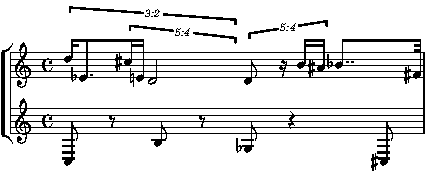
\includegraphics{assets/lilypond-8d72e9a5aced38c13d509aea16c53ca6.pdf}
%%% ABJADBOOK END %%%

Composers can attach spanners (such as ties and slurs) to score components via
Abjad's top-level \texttt{attach()} function.

\begin{comment}
<abjad>
upper_leaves = upper_staff.select_leaves()
lower_leaves = lower_staff.select_leaves()
attach(Tie(), upper_leaves[4:6])
attach(Tie(), upper_leaves[-3:-1])
attach(Slur(), upper_leaves[:2])
attach(Slur(), upper_leaves[2:6])
attach(Slur(), upper_leaves[7:])
</abjad>
\end{comment}

%%% ABJADBOOK START %%%
\begin{lstlisting}
>>> upper_leaves = upper_staff.select_leaves()
>>> lower_leaves = lower_staff.select_leaves()
>>> attach(Tie(), upper_leaves[4:6])
>>> attach(Tie(), upper_leaves[-3:-1])
>>> attach(Slur(), upper_leaves[:2])
>>> attach(Slur(), upper_leaves[2:6])
>>> attach(Slur(), upper_leaves[7:])
\end{lstlisting}
%%% ABJADBOOK END %%%

Composers can also attach indicators (such as articulations and clefs) to
individual score components with \texttt{attach()}.

\begin{comment}
<abjad>
attach(Articulation('accent'), upper_leaves[0])
attach(Articulation('accent'), upper_leaves[2])
attach(Articulation('accent'), upper_leaves[7])
attach(Clef('bass'), lower_leaves[0])
show(score)
</abjad>
\end{comment}

%%% ABJADBOOK START %%%
\begin{lstlisting}
>>> attach(Articulation('accent'), upper_leaves[0])
>>> attach(Articulation('accent'), upper_leaves[2])
>>> attach(Articulation('accent'), upper_leaves[7])
>>> attach(Clef('bass'), lower_leaves[0])
>>> show(score)
\end{lstlisting}
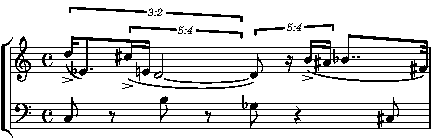
\includegraphics{assets/lilypond-6e6234ddf98e707d42a58b6306767fc8.pdf}
%%% ABJADBOOK END %%%

Combining score components piece by piece into ever-larger aggregates gives
composers fine-grained control over their compositional structures. Such
control guarantees a high degree of compositional-process agnosticism on
Abjad's part, and affords composers a solid framework on top of which they can
design and implement their own personal approaches to composition.

\section{Input flexibility}

We believe that there should be multiple ways of instantiating compositional
elements. Input flexibility affords composers the ability to create
compositional objects in whatever way closest aligns with their conception of
music and their specific task at hand \cite{Kay:1996vn}. Abjad's score
components can be created in a variety of ways. Leaves (such as notes) can be
instantiated parametrically by specifying pitch and rhythm information
numerically. Leaves can also be created via explicit \texttt{Pitch} and
\texttt{Duration} objects. Containers (such as tuplets and measures) can be
instantiated parametrically by specifying explicit lists of components to be
inserted as children. Abjad also allows many score objects to be created via
strings parseable in one of the various micro-languages we have implemented.
Score components created via string input can be potentially much more complex
than those created parametrically because Abjad's microlanguage parsers have
the ability to attach spanners and indicators to the created components or
their children, if they are containers. Parametric instantiation affords
composers powerful procedural control over score structure while string
instantiation allows for brevity and expressiveness. The score construction
example above demonstrates both techniques.

\section{Top-down construction} \label{sec:top-down}

With experience, use of the system migrates from bottom-up to top-down. We
realize that composers probably don't find it interesting to make a single
note, but can be deeply engaged by the process of creating intermediate and
high-level objects like phrases or complete segments of music. Abstraction,
encapsulation and re-use of generative processes is what comes closest to the
work of beginning to implement one's own system of composition.

\subsection{Factory functions, factory classes}

Abjad provides a variety of factories for quickly and flexibly creating
arbitrarily large amounts of notation. These range from simple leaf-generating
functions like \texttt{make\_notes()}, which
combine sequences of pitches and rhythms isorhythmically to generate selections
of notes and rests, to more complexly-configured \emph{maker} classes for
creating nuanced rhythmic patterns or entire scores.

\begin{comment}
<abjad>
notes = scoretools.make_notes([0, 1, 4, 7], [(1, 4)],)
staff = Staff(notes)
show(staff)
</abjad>
\end{comment}

%%% ABJADBOOK START %%%
\begin{lstlisting}
>>> notes = scoretools.make_notes([0, 1, 4, 7], [(1, 4)],)
>>> staff = Staff(notes)
>>> show(staff)
\end{lstlisting}
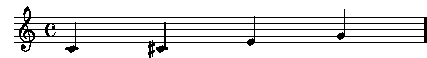
\includegraphics{assets/lilypond-64155bcaa384109d40ae2616a2224dd1.pdf}
%%% ABJADBOOK END %%%

Abjad's \emph{rhythm makers} are factory classes which, once configured, can be
called like functions to procedurally inscribe rhythms into a series of
\emph{divisions}. The \texttt{NoteRhythmMaker} fills in divisions with notes,
tied as necessary, to equal the duration of those divisions.

\begin{comment}
<abjad>
divisions = [(3, 8), (5, 16), (1, 4), (3, 16)]
rhythm_maker = rhythmmakertools.NoteRhythmMaker()
show(rhythm_maker, divisions=divisions)
</abjad>
\end{comment}

%%% ABJADBOOK START %%%
\begin{lstlisting}
>>> divisions = [(3, 8), (5, 16), (1, 4), (3, 16)]
>>> rhythm_maker = rhythmmakertools.NoteRhythmMaker()
>>> show(rhythm_maker, divisions=divisions)
\end{lstlisting}
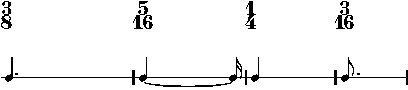
\includegraphics{assets/lilypond-af2aa88dc88360a6a0cf5c3f8da17b85.pdf}
%%% ABJADBOOK END %%%

Other rhythm makers, such as Abjad's \texttt{TaleaRhythmMaker}, can create even
more complex rhythmic output, integrating configurable patterns of durations,
tupletting and silences.

\begin{comment}
<abjad>
rhythm_maker = rhythmmakertools.TaleaRhythmMaker(
    burnish_specifier=rhythmmakertools.BurnishSpecifier(
        left_classes=(Rest, Note),
        left_counts=(1,),
        ),
    extra_counts_per_division=(0, 1, 1),
    talea=rhythmmakertools.Talea(
        counts=(1, 2, 3),
        denominator=16,
        ),
    tie_specifier=rhythmmakertools.TieSpecifier(
        tie_across_divisions=True,
        ),
    )
show(rhythm_maker, divisions=divisions)
</abjad>
\end{comment}

%%% ABJADBOOK START %%%
\begin{lstlisting}
>>> rhythm_maker = rhythmmakertools.TaleaRhythmMaker(
...     burnish_specifier=rhythmmakertools.BurnishSpecifier(
...         left_classes=(Rest, Note),
...         left_counts=(1,),
...         ),
...     extra_counts_per_division=(0, 1, 1),
...     talea=rhythmmakertools.Talea(
...         counts=(1, 2, 3),
...         denominator=16,
...         ),
...     tie_specifier=rhythmmakertools.TieSpecifier(
...         tie_across_divisions=True,
...         ),
...     )
>>> show(rhythm_maker, divisions=divisions)
\end{lstlisting}
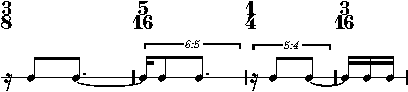
\includegraphics{assets/lilypond-cf8687c5463d3d6aec12827476c8fc4e.pdf}
%%% ABJADBOOK END %%%

Once instantiated, rhythm makers can be used over and over again with different
input, a pattern used pervasively in Abjad: maker classes as object-oriented
partially-evaluated functions. As generating duration sequences is generally
less difficult than creating complete tupletted, beamed and tied rhythmic score
artifacts, rhythm makers allow composers to focus on the process of building
rhythm structures as a compositional material in-and-of itself. Because rhythm
makers are classes, they can be subclassed and extended in order to modify
their behavior. Because they are objects, they can be passed as parameters to
configure even more expansive aggregate makers.

\emph{Score templates} are another common factory pattern in Abjad,
encapsulating the work of building the skeletons of complete scores, including
voices, staves, staff groups, clefs and other indications pertinent to the
intended instrumentation or typography. We can combine rhythm and score makers
with score iteration, as well as some simple bottom-up construction, to
generate complete score aggregates expressively.

\begin{comment}
<abjad>
template = templatetools.\
    GroupedRhythmicStavesScoreTemplate(4)
quartet_score = template()
iterator = iterate(quartet_score).by_class(Voice)
for index, voice in enumerate(iterator):
    divisions = sequencetools.rotate_sequence(
        divisions, -1)
    selections = rhythm_maker(divisions, seeds=-index)
    measure = Measure((9, 8), selections)
    voice.append(measure)

show(quartet_score)
</abjad>
\end{comment}

%%% ABJADBOOK START %%%
\begin{lstlisting}
>>> template = templatetools.\
...     GroupedRhythmicStavesScoreTemplate(4)
>>> quartet_score = template()
>>> iterator = iterate(quartet_score).by_class(Voice)
>>> for index, voice in enumerate(iterator):
...     divisions = sequencetools.rotate_sequence(
...         divisions, -1)
...     selections = rhythm_maker(divisions, seeds=-index)
...     measure = Measure((9, 8), selections)
...     voice.append(measure)
...
>>> show(quartet_score)
\end{lstlisting}
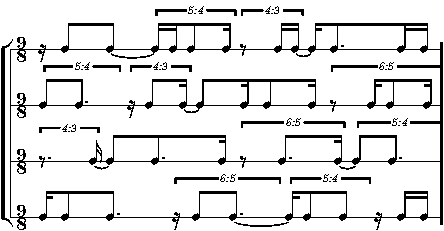
\includegraphics{assets/lilypond-07f633b33deadb5b938f688d727585f0.pdf}
%%% ABJADBOOK END %%%

\subsection{Top-down extensibility}

We believe that there are more ways to generate notation than we can conceive
of. While Abjad has implemented many notational factories, we do not think
these are sufficient for any one artist's process and have therefore
architected the project in such a way as to encourage extension by composers
interacting with the system in the spirit of compositional agnosticism.

\subsection{Templating}

As demonstrated earlier, Abjad's \emph{rhythm makers} are highly-configurable
factory classes for generating rhythmic patterns. Many of their initialization
keywords expect \emph{specifiers} --- object-oriented bundles of related
parameters --- which can make their configurations potentially deeply nested.

\begin{comment}
<abjad>
rhythm_maker = rhythmmakertools.TaleaRhythmMaker(
    talea=rhythmmakertools.Talea(
        counts=(1, 2, 3),
        denominator=16,
        ),
    )
print(format(rhythm_maker))
</abjad>
\end{comment}

%%% ABJADBOOK START %%%
\begin{lstlisting}
>>> rhythm_maker = rhythmmakertools.TaleaRhythmMaker(
...     talea=rhythmmakertools.Talea(
...         counts=(1, 2, 3),
...         denominator=16,
...         ),
...     )
>>> print(format(rhythm_maker))
rhythmmakertools.TaleaRhythmMaker(
    talea=rhythmmakertools.Talea(
        counts=(1, 2, 3),
        denominator=16,
        ),
    )
\end{lstlisting}
%%% ABJADBOOK END %%%

\begin{comment}
<abjad>
divisions = [(3, 8), (1, 4), (5, 16), (1, 4)]
show(rhythm_maker, divisions=divisions)
</abjad>
\end{comment}

%%% ABJADBOOK START %%%
\begin{lstlisting}
>>> divisions = [(3, 8), (1, 4), (5, 16), (1, 4)]
>>> show(rhythm_maker, divisions=divisions)
\end{lstlisting}
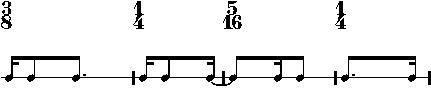
\includegraphics{assets/lilypond-8d11397fa8a7ed768182e6c89abe52f0.pdf}
%%% ABJADBOOK END %%%

Nested configuration via parameter grouping with specifiers provides
considerable conceptual clarity, but is also potentially labor-intensive. Abjad
mitigates the work of complex configuration by affording composers with
powerful templating tools. New objects can be created from old ones, optionally
replacing any initialization parameter in the templated object at any depth via
the top-level \texttt{new()} function. Notice how the new rhythm maker below
has both altered its talea counts and added a new initialization keyword.

\begin{comment}
<abjad>
new_rhythm_maker = new(rhythm_maker,
    extra_counts_per_division=(0, 1),
    talea__counts=(1, 2, 3, 4),
    )
print(format(new_rhythm_maker))
</abjad>
\end{comment}

%%% ABJADBOOK START %%%
\begin{lstlisting}
>>> new_rhythm_maker = new(rhythm_maker,
...     extra_counts_per_division=(0, 1),
...     talea__counts=(1, 2, 3, 4),
...     )
>>> print(format(new_rhythm_maker))
rhythmmakertools.TaleaRhythmMaker(
    talea=rhythmmakertools.Talea(
        counts=(1, 2, 3, 4),
        denominator=16,
        ),
    extra_counts_per_division=(0, 1),
    )
\end{lstlisting}
%%% ABJADBOOK END %%%

\begin{comment}
<abjad>
show(new_rhythm_maker, divisions=divisions)
</abjad>
\end{comment}

%%% ABJADBOOK START %%%
\begin{lstlisting}
>>> show(new_rhythm_maker, divisions=divisions)
\end{lstlisting}
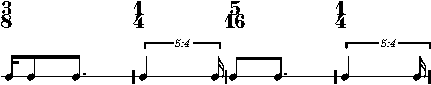
\includegraphics{assets/lilypond-a769357ad75c64d981f789b0e3a0f4da.pdf}
%%% ABJADBOOK END %%%

Repeating the templating process creates new and different yet still related
objects, allowing composers to easily play with variation at the level of
procedure.

\begin{comment}
<abjad>
new_new_rhythm_maker = new(new_rhythm_maker,
    extra_counts_per_division=(0, 1, 2),
    beam_specifier=rhythmmakertools.BeamSpecifier(
        beam_divisions_together=True,
        ),
    )
print(format(new_new_rhythm_maker))
</abjad>
\end{comment}

%%% ABJADBOOK START %%%
\begin{lstlisting}
>>> new_new_rhythm_maker = new(new_rhythm_maker,
...     extra_counts_per_division=(0, 1, 2),
...     beam_specifier=rhythmmakertools.BeamSpecifier(
...         beam_divisions_together=True,
...         ),
...     )
>>> print(format(new_new_rhythm_maker))
rhythmmakertools.TaleaRhythmMaker(
    talea=rhythmmakertools.Talea(
        counts=(1, 2, 3, 4),
        denominator=16,
        ),
    extra_counts_per_division=(0, 1, 2),
    beam_specifier=rhythmmakertools.BeamSpecifier(
        beam_each_division=True,
        beam_divisions_together=True,
        ),
    )
\end{lstlisting}
%%% ABJADBOOK END %%%

\begin{comment}
<abjad>
show(new_new_rhythm_maker, divisions=divisions)
</abjad>
\end{comment}

%%% ABJADBOOK START %%%
\begin{lstlisting}
>>> show(new_new_rhythm_maker, divisions=divisions)
\end{lstlisting}
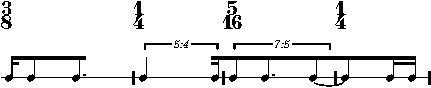
\includegraphics{assets/lilypond-23e2752f7db7cf02e31cf8e9f399c5b6.pdf}
%%% ABJADBOOK END %%%

%By providing core functionality oriented toward the elements of standard
%notation, Abjad strives to remain as agnostic as possible to various
%composition techniques.

\section{Selection flexibility} \label{sec:selections}

we think it's important for composers to be able to select arbitrary
collections of score objects. this is important for a couple of reasons. first,
so that composers can map operations to the entirety of such a selection at one
time. second, there's some type of conceptual benefit to be had in named
selections; the point is that every selection is an ad hoc intermediate
structure created in the midst of the score. we also think it's important to
afford composers the ability to reference score objects in whatever ways are
most natural for a given task. sometimes the most natural mode of reference is
numeric, sometimes by name or sometimes by music-specific criteria such as the
relative times at which different objects appear in the score. examples follow.
we provide concrete object models of vertical relationships in the score.

selecting one object: by number, by time relation, by name.

selecting many things: by slicing, by select\_leaves(), by iteration.

[TREVOR]

%Abjad allows the numeric addressing of all score components. Abjad score
%components are zero-indexed from the start of the container which holds them:
%the statement \texttt{staff[0]} addresses the first component contained in
%\texttt{staff} while the statement \texttt{staff[1]} addresses the component
%after that, and so on. Negative indices address components from the end of the
%container which holds them. Python's slice notation may be used to retrieve an
%arbitrary number of contiguous components at one time. As an example of the
%latter, the statement \texttt{staff[15:25]} selects the ten components in
%\texttt{staff} between indices 15 and 25. The conventions of Abjad's numeric
%addressing regime follow those of Python's list and tuple interface exactly.

Consider the two-staff score created earlier. The upper staff can be selected
by indexing the first child of the first child of the score, i.e. the first
staff in the staff group which is the first child of the score itself.

\begin{comment}
<abjad>
upper_staff = score[0][0]
show(upper_staff)
</abjad>
\end{comment}

%%% ABJADBOOK START %%%
\begin{lstlisting}
>>> upper_staff = score[0][0]
>>> show(upper_staff)
\end{lstlisting}
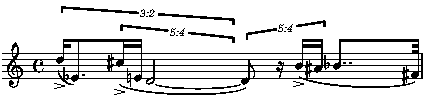
\includegraphics{assets/lilypond-4aa1bd58533df74ce54d499ffd6dbb25.pdf}
%%% ABJADBOOK END %%%

Because both staves were given explicit names, they can also be selected by
those names, regardless of their depth in the score hierarchy.

\begin{comment}
<abjad>
lower_staff = score['Lower Staff']
show(lower_staff)
</abjad>
\end{comment}

%%% ABJADBOOK START %%%
\begin{lstlisting}
>>> lower_staff = score['Lower Staff']
>>> show(lower_staff)
\end{lstlisting}
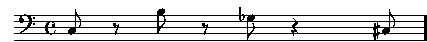
\includegraphics{assets/lilypond-fa746e527d218a814e36af2f46d314bb.pdf}
%%% ABJADBOOK END %%%

A score container's leaves --- the notes, chords and rests at the bottom of the
score hierarchy which cannot, by definition, contain any other score component
--- can be selected by that container's \texttt{select\_leaves()} method.

\begin{comment}
<abjad>
for leaf in lower_staff.select_leaves():
    print(repr(leaf))

</abjad>
\end{comment}

%%% ABJADBOOK START %%%
\begin{lstlisting}
>>> for leaf in lower_staff.select_leaves():
...     print(repr(leaf))
...
Note('c8')
Rest('r8')
Note('b8')
Rest('r8')
Note('gf8')
Rest('r4')
Note('cs8')
\end{lstlisting}
%%% ABJADBOOK END %%%

Composers can select components via Abjad's powerful top-level
\texttt{iterate()} function, which exposes the score iteration interface as
implemented in our \texttt{IterationAgent}. The iteration interface affords a
wide variety of selection criteria, such as class filters, logical tie
selection and time-wise score traversal.

\begin{comment}
<abjad>
for note in iterate(lower_staff).by_class(Note):
    attach(Articulation('staccato'), note)

show(score)
</abjad>
\end{comment}

%%% ABJADBOOK START %%%
\begin{lstlisting}
>>> for note in iterate(lower_staff).by_class(Note):
...     attach(Articulation('staccato'), note)
...
>>> show(score)
\end{lstlisting}
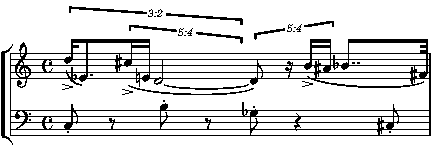
\includegraphics{assets/lilypond-85c47ec39685eb2a539925a3599691c2.pdf}
%%% ABJADBOOK END %%%

\begin{comment}
<abjad>
iterator = iterate(score).by_logical_tie(
    nontrivial=True, pitched=True)
for logical_tie in iterator:
    attach(Fermata(), logical_tie.tail)

show(score)
</abjad>
\end{comment}

%%% ABJADBOOK START %%%
\begin{lstlisting}
>>> iterator = iterate(score).by_logical_tie(
...     nontrivial=True, pitched=True)
>>> for logical_tie in iterator:
...     attach(Fermata(), logical_tie.tail)
...
>>> show(score)
\end{lstlisting}
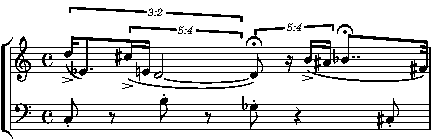
\includegraphics{assets/lilypond-1981e2f1300698407cb416bc14b38c23.pdf}
%%% ABJADBOOK END %%%

\begin{comment}
<abjad>
iterator = iterate(score).by_timeline()
for index, component in enumerate(iterator):
    markup = Markup(index, Up).box()
    attach(markup, component)

show(score)
</abjad>
\end{comment}

%%% ABJADBOOK START %%%
\begin{lstlisting}
>>> iterator = iterate(score).by_timeline()
>>> for index, component in enumerate(iterator):
...     markup = Markup(index, Up).box()
...     attach(markup, component)
...
>>> show(score)
\end{lstlisting}
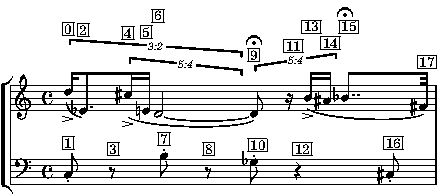
\includegraphics{assets/lilypond-783949753898126e596d11728f72bf61.pdf}
%%% ABJADBOOK END %%%

\section{Open-source best practices} \label{sec:open-source}

The architecting of Abjad has benefited enormously from programming best
practices developed by the open-source community. One of these best practices
--- the principle of extending an existing language rather than building from
the ground up --- is so important that we introduced it earlier as a first
principle behind our work. In this section we list other best practices we have
taken from the open-source community and discuss the ways these principles
impact the development of music software systems.

\subsection{Automated regression testing}

The music software systems academic literature we have investigated is
overwhelmingly silent on questions of software testing. None of the sources
cited in this article reference software test methodologies. The same appears
to be true for the larger list of sources included in
\cite{trevino2013compositional}.\footnote{Chris Ariza's work developing
AthenaCL [SOURCE] and the development of Music21 [SOURCE] led by Michael
Cuthbert are important exceptions. Both projects are implemented in Python and
both projects feature approaches to testing aligned to those outlined above.}
Why should this be the case? One possibility is that authors of music software
systems have, in fact, availed themselves of important improvements in software
test methods developed over the previous decades but have, for whatever
reasons, remained quiet on the matter in the publication record. We think a
more likely explanation is that the culture of software best practices now
widely followed in the open-source community simply has not yet arrived in the
field of music software systems development (and especially in the development
of music software systems designed for noncommercial applications).

Our experience developing Abjad leads us to believe that the focus on testing
absent the majority of music software systems is a liability to the field in
two ways.\footnote{Abjad comprises an automated battery of 9,119 unit tests and
8,528 documentation tests. Unit tests are executed by \texttt{pytest}.
Documentation tests are executed by the \texttt{doctest} module included in
Python's standard library. Parametrized tests are provided to ensure that
behaviors implemented the same way against different classes produce
corresponding output. Developers run the entire battery of tests at the start
of every development session. No new features are accepted as part of the Abjad
codebase without tests authored to document changes to the system. Continuous
integration testing is handled by Travis CI to ensure that nightly builds of
Abjad installed under different operating systems continue to pass all tests.
For \texttt{pytest} see \textit{http://pytest.org}. For Travis CI see
\textit{https://travis-ci.org}.}

The first such liability concerns systems development. The absence of automated
regression tests acts as a barrier to new contributors to the system (who
effectively have no way to determine whether proposed changes to the system
negatively impact the system) and severely attenuates the rate at which
experienced developers can refactor the system during new feature development.
Consider that Abjad currently comprises about 178,000 lines of code and that
the Abjad repository hosted on GitHub\footnote{https://github.com/Abjad/abjad}
lists more than 8.7 million lines of code committed since the start of the
project. This refactor ratio of about 50:1 means that each line of code in the
Abjad codebase has been rewritten dozens of times. This freedom to refactor is
possible only because of the approach to automated regression testing we have
borrowed from the larger open-source community.

The second testing-related liability we diagnose concerns project continuance.
What happens when the original developers of a music software system are no
longer available to develop the system? Automated regression tests help make
possible a changing of the guard from one set of developers to another. This is
true because automated tests serve as a type of functional specification of how
a software system is supposed to behave after the system is altered. While
automated tests alone will not ensure the continued development of any software
system, we believe that adherence to the testing practices of the open-source
community constitutes the most effective hedge available to music software
systems developers to fend against project abandonment in the medium and long
term.

\subsection{Extensibility}

As an open-source project, composers and researchers can contribute changes via
git pull requests. A process of continuous integration and online version
control simplifies this contribution process.

\subsection{Embeddability}

Abjad is an importable Python library. It can be used in whole or in part as a
component of any Python-compatible system. Abjad has few Python package
dependencies and is not bound to any specific user application or graphic user
interface. These qualities make Abjad an ideal project ideal for embedding in
other software systems.

For example, Abjad supports IPython
Notebook\footnote{http://ipython.org/notebook.html}, a web-based interactive
computational environment combining code execution, text, mathematics, plots
and rich media into a single document. Notational output from Abjad can be
transparently captured and embedded directly into an IPython Notebook which has
loaded Abjad's IPython Notebook extension. Calls to Abjad's \texttt{show()} are
intercepted and the rendered graphics are embedded directly into the Notebook
along with the generating code. This allows scholars to quickly and intuitively
create music texts which can be shared, edited and executed by other IPython
users.

\subsection{Maintainability}

Text here.

extensive documentation

community coding standards

distributed version control

\section{conclusion} \label{sec:conclusion}

we want composers to become programmers. for extremely good reasons. and the
priorities we have detailed here help make the case for why. [TREVOR]

\bibliography{tenor2015}
\end{document}